% Asset ID: A22NormalDistributionTIKZ-004
% Source: Phase 1 Core Theory Part 3
% Related lesson section: Core Theory Part 3
% Purpose: Inverse normal left-tail area, find boundary a
\documentclass[tikz,border=8pt]{standalone}
\usepackage{amsmath}
\usepackage{tikz}
\usetikzlibrary{arrows.meta,calc}
\begin{document}
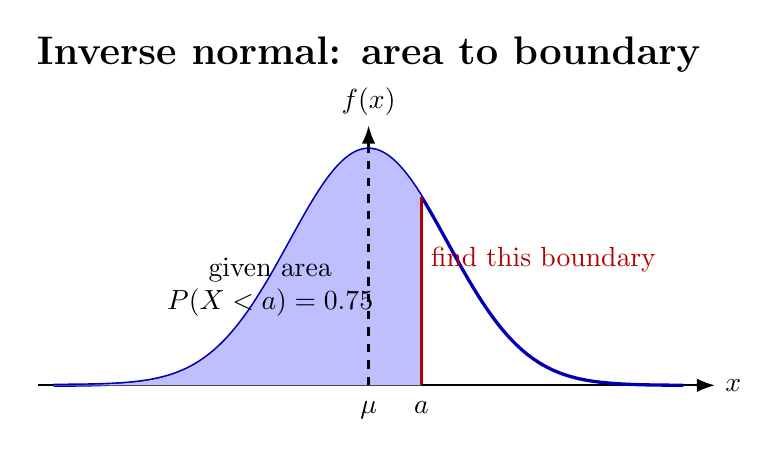
\begin{tikzpicture}[x=1cm,y=1cm,>=Latex]
\node[font=\Large\bfseries] at (0,4.2) {Inverse normal: area to boundary};
\draw[->, thick] (-4.2,0) -- (4.4,0) node[right] {$x$};
\draw[->, thick] (0,0) -- (0,3.3) node[above] {$f(x)$};
\draw[very thick, blue!70!black, domain=-4:4, samples=250] plot (\x,{3*exp(-0.5*\x*\x)});
\def\a{0.67}
\fill[blue!25, domain=-4:\a, samples=200] plot (\x,{3*exp(-0.5*\x*\x)}) -- (\a,0) -- (-4,0) -- cycle;
\draw[dashed, thick] (0,0) -- (0,3);
\draw[very thick, red!70!black] (\a,0) -- (\a,{3*exp(-0.5*\a*\a)});
\node[below] at (0,-0.08) {$\mu$};
\node[below] at (\a,-0.08) {$a$};
\node[align=center] at (-1.25,1.25) {given area\\$P(X<a)=0.75$};
\node[red!70!black, right] at (\a,{1.6}) {find this boundary};
\end{tikzpicture}
\end{document}
